\cotefile{12}
\scanpage{64}
% Three vertical emphasis strokes to the left of lines 1–3.
soient des isomorphismes, avec % 1
le complément que $H^*(X,M)$ \uline{est un} % 2
$\mathbb{Q}$-\uline{\deleted{\unsure{m}}module de type fini}. \deleted{Ceci doit être % 3
valable en particulier dans les deux % 4
cas types suivants % 5

a) $X$ de type fini sur $\mathbb{Z}$ % 6

b) $X$ de type fini sur un corps % 7
alg. clos.} % 8

En particulier, pour un corps alg. clos $k$, on % 9
aura $H^i(k,M)=0$ pour $i>0$, $\forall$ motif $M$. % 10

\uline{NB} Si $X$ est de type fini (ou projectif lisse) % 11
sur un corps alg. clos $K$, on \unsure{n'a} plus de % 12
telles relations précises, comme on voit % 13
par calcul \unsure{confiant|cofini|explicite} (utilisant les conjectures % 14
de Tate) pour $K$ clôture algébrique % 15
d'un corps fini ---- % 16

Le th de Tate permet de reformuler et % 17
se préciser en énonçant : % 18
\[
 A^i(X)\otimes_{\mathbb{Z}}\overset{\inserted{\nearrow\,\text{pas}\,\mathbb{Q}_{\ell}}}{\mathbb{Q}}
 \simeq\Gamma_k\bigl(R^i f_*(\mathbb{Q}_X(0))\bigr) % 19
\]
% archive sheet number: 63
\scanpage{65}
$X$ étant projectif et lisse sur $k$ alg. clos, % 1
morphisme structural $f:X\longrightarrow\operatorname{Spec} k$. % 2
Une autre façon est celle-ci % 3
\[
 \boxed{A^i(X)\deleted{\otimes_{\mathbb{Z}}\mathbb{Q}}\simeq
 \operatorname{Im}\bigl[H^{2i}(X,\mathbb{Q}(i))\longrightarrow
 H^{2i}(X,\mathbb{Q}_{\ell}(i))\bigr]} % 4
\]

\uline{NB.} Si $k$ est la clôture algébrique % 5
de $\mathbb{F}_p$, on \unsure{trouve} pour $X$ projectif lisse sur % 6
$k$ % 7
\[
\begin{aligned}
H^{\deleted{\unsure{2i}}i}(X,\overset{\inserted{\nearrow\,\text{\uuline{pas} }\mathbb{Q}_{\ell}(i)!}}{\mathbb{Q}}(j))
={}&\left\{\begin{aligned}
&0 &&\text{si }\unsure{i|j}\ne 2j,2j+1\\ % 8
&A^{\unsure{i|j}}(X)\otimes_{\mathbb{Z}}\mathbb{Q}
 &&\text{si }i=2j\\ % 9
& &&\text{(canonique)}\\ % 10
&A^{\unsure{j|i}}(X)\otimes_{\mathbb{Z}}\mathbb{Q}
 &&\text{si }i=j+1\\ % 11
& &&\text{(\uline{pas} canonique)}
\end{aligned}\right. % 12
\end{aligned}
\]
De plus, pour $i\ne 2j$, l'image de % 13
$H^i(X,\mathbb{Q}(j))$ dans $H^i(X,\mathbb{Q}_{\ell}(j))$ est nulle. % 14

C'est \uline{un fait général} : si $k$ alg. % 15
clos, alors (si $X$ projectif lisse sur $k$) l'image % 16
de $H^{\deleted{\unsure{2i}}j}(X,\mathbb{Q}(\deleted{\unsure{j}}i))\to H^j(X,\mathbb{Q}_{\ell}(i))$ % 17
est \uline{nulle} pour $j\ne 2i$ (question de % 18
poids) ; pour $j=2i$ ce sont les cycles % 19
algébriques \inserted{à coeff} rationnels. % 20
% archive sheet number: 64
\scanpage{67}
Notons le \uline{th. de dualité absolue} : % 1
Soient $M$ et $M^*$ deux \inserted{(complexes de)} motifs sur % 2
$X$ (de type fini sur $\mathbb{Z}$), qui sont % 3
\textquotedblleft duals\textquotedblright{} pour le \deleted{\unsure{\textup{[}}}complexe de motifs % 4
dualisant\deleted{\unsure{s}}\deleted{\unsure{\textup{]}}} canonique -- [NB. Si $X$ % 5
est régulier \inserted{partout} de dim $n$, alors % 6
c'est la dualité à valeurs \deleted{dans $\unsure{\mathbb{Q}(n)[\,]| \mathbb{Q}(n)[2n]}$ shift} \inserted{$\mathbb{Q}(n)[2n+1]$}\margin{shift}] % 7

alors $\mathbb{R}\Gamma_X(M)$ et $\mathbb{R}_!\Gamma_X(M^*)$\margin{\textquotedblleft support cpt sur $\operatorname{Spec}\mathbb{Z}$\textquotedblright} sont % 8
duals. Ici [Comme les coefficients sont % 9
ess. $\mathbb{Q}$\deleted{\unsure{s|\textup{\}}}}, donc il n'y a pas de $\operatorname{Tor}$] % 10
ceci revient aussi à la formule (cas régulier) % 11
\[
\boxed{\begin{aligned}
H^i(X,M)&\quad\text{dual de}\quad\operatorname{Ext}^{2n+1-i}_!(X;M,\mathbb{Q}(n))\\ % 12
H^i_!(X,M)&\quad\text{dual de}\quad\operatorname{Ext}^{2n+1-i}(X;M,\mathbb{Q}(n)) % 13
\end{aligned}}
\]
Si $X$ propre sur $\operatorname{Spec}\mathbb{Z}$, inutile de mettre % 14
des $!$. % 15

Moyennant le \unsure{thm|th.} de dualité \uline{relative} % 16
pour motifs, cet énoncé revient au % 17
% archive sheet number: 66
\scanpage{71}
$X$ projective lisse \inserted{géom. connexe} sur $k$ corps fini à $q$ éléments. % 1

Par passage à la limite sur les \deleted{quotients} \inserted{coefficients} finis, on % 2
trouve % 3
\[
0\to H^{i-1}(\bar X,\mathbb{Q}_{\ell}(j))_{\pi}
\longrightarrow H^i(\deleted{\unsure{\overline{\phantom X}}}X,\mathbb{Q}_{\ell}(j))
\longrightarrow H^i(\bar X,\mathbb{Q}_{\ell}(j))_{\deleted{\unsure{\pi}}}^{\pi}\to 0 % 4
\]
d'où le résultat % 5
\[
\begin{aligned}
\text{si } i\ne2j,2j+1,\qquad & H^i(X,\mathbb{Q}_{\ell}(j))=0\\ % 6
\text{Si } i=2j\qquad & H^{\deleted{\unsure{i}}2j}(X,\mathbb{Q}_{\ell}(j))
 = H^{2j}(\bar X,\mathbb{Q}_{\ell}(j))^{\pi}\\ % 7
&\hspace{38mm}\rotatebox{90}{$\simeq$}\ \text{Conj. de Tate}\\ % 8
&\hspace{34mm} A^j(X/k)\otimes_{\deleted{\mathbb{Q}}\mathbb{Z}}\mathbb{Q}_{\ell}\\ % 9
\text{si } i=2j+1\qquad & H^{2j+1}(X,\mathbb{Q}_{\ell}(j))
 =H^{2j\deleted{\unsure{+1}}}(\bar X,\mathbb{Q}_{\ell}(j))_{\pi}\\ % 10
&\hspace{38mm}\rotatebox{90}{$\simeq$}\ \text{Tate + action semi-simple}\\ % 11
&\hspace{34mm} A^j(X/k)\otimes_{\deleted{\mathbb{Q}}\mathbb{Z}}\mathbb{Q}_{\ell}
\end{aligned} % 12
\]
Soit maintenant $k_n$ l'extension de degré % 13
$n$ de $k$ dans $\bar k$, et étudions % 14
\[
\varinjlim_n H^i(X_{k_n},\mathbb{Q}_\ell(j)) % 15
\]
On trouve $0$ pour $i\ne2j,2j+1$ ; pour % 16
$i=2j$, on trouve $H^{2j}(\bar X,\mathbb{Q}_{\ell}(j))^{\unsure{oj|of|0j|\mathfrak{g}}}=A^j(\bar X)\otimes_{\deleted{\mathbb{Q}}\mathbb{Z}}\mathbb{Q}_{\ell}$, % 17
enfin pour $i=2j+1$, on trouve également % 18
$A^j(\bar X)\otimes_{\mathbb{Z}}\mathbb{Q}_{\ell}$. \deleted{\unsure{Donc|De}} \unsure{on|$=$}, on trouve \inserted{du pt de vue motifs} % 19
\[
\begin{aligned}
\varinjlim H^i(X_{k_{\unsure{n|\infty}}},\mathbb{Q}(j))
&=\left\{\begin{aligned}
&0 &&\text{si }i\ne2j,2j+1\\ % 20
&A^j(\bar X)\otimes_{\deleted{\mathbb{Q}}\mathbb{Z}}\mathbb{Q}&&\text{si }i=2j\deleted{,2j+1}\\ % 21
&\deleted{\unsure{A^j(\bar X)\otimes\mathbb{Q}}}\ \text{id}&&\text{si }i=2j+1,
\end{aligned}\right.\\ % 22
\rotatebox{90}{$=$}\qquad&\hspace{17mm}\text{mais pas \uline{canoniquement} en}\\ % 23
H^i(\bar X,\mathbb{Q}(j))\qquad&\hspace{17mm}\text{\unsure{donnant|donnons|termes} un }\unsure{\bar x|x|\bar X},\ \bar\pi\,!
\end{aligned} % 24
\]
\margin{\uline{N.B.} \unsure{Remplaçons|Remplacer} $k$ par $k_n$ revient à multiplier l'isom obtenu par $\unsure{n'/n|n/n|1/n}$ ---} % 25
% archive sheet number: 70
\scanpage{72}
% Typescript upside down relative to the scan. A single pen stroke cancels the block.
\deleted{Ceci donne une démonstration plus sympatique et élémentaire de % 1
11.9.5. Quant à 11.9.3. (ii), il varésulter d'un % 2

\uline{Lemme} (ou cor\deleted{\unsure{a|o}}ollaire à la proposition précédente). Sous les \unsure{hypothèse|hypothèses} % 3
de la proposition, ne supposons plus néc que $A'$ soit projectif sur $A$, % 4
mais seulement ceci: pour tout quotient intègre $B=A/\underline p$ de $A$, posant % 5
$B'=B\otimes_A A'$, il existe un $h\quad B-(0)$ tel que $B_h$ soit \deleted{projectif} \inserted{libre} sur $A_h$. % 6
Alors la conclusion de la proposition reste encore valable. % 7

Soit en effet $\phi$ une section de $F'$ dont les images par les % 8
$u'$ sont nulles, prouvons $\phi=0$, i.e. $\operatorname{supp}\phi=\emptyset$. Dans le cas contraire, % 9
il existerait un point maximal $x'$ dans $\operatorname{supp}\phi$, correspondant % 10
à l'idéal premier $\underline p'$ de $A'$. Soit \deleted{$\underline p=\underline p'\unsure{\cap A'|\cap A}$} \inserted{$x$} son image dans $X$, défini % 11
par l'idéal $\underline p$ trace de $\underline p'$ sur $A$, alors en vertu de l'hypothèse % 12
appliquée à $A/\underline p$, on voit que, quitte à remplacer $X$ par un voisinage % 13
ouvert affine de $x$, on peut supposer que $\deleted{\unsure{A}}B'/\underline p\deleted{\unsure{A}}B'$ est \deleted{projectif} \inserted{libre} sur % 14
$A/\underline p$. Notons que nous pouvions choisir $x'$ de façon que $x$ soit également % 15
maximal dans $g(\operatorname{supp}\phi)$ (commencer par choisir $x$ maximal dans % 16
$g(\operatorname{supp}\phi)$, puis $x'$ maixmal dans $g^{-1}(x)$ ), ce qui signifie que % 17
localisant en $\underline p$, le support de $\phi_{\underline p}$ est contenu dans $\operatorname{Spec}(A'_{\underline p}/\underline p A'_{\underline p})$, % 18
donc $\phi_{\underline p}$ est annulé par une puissance de $\underline p A'_{\underline p}$, ou encore que % 19
l'on peut trouver $h\quad A-\underline p$ tel que} % 20
% archive sheet number: 71
\scanpage{73}
$S$ \inserted{lisse} de \deleted{\unsure{f}} type fini sur $\mathbb{F}_p$ % 1

$M$ motif ct tordu de poids $\rho$ % 2
\[
 ?\;-\; H^*(S,M_\ell)\overset{?}{\Leftarrow}
 H^p(\mathbb{F}_p,R^q f_*(M_\ell)) % 3
\]
\[
\begin{aligned}
0\to{}&
\underbrace{H^{\unsure{i-1|i}}(\bar S,\bar M_\ell)_{\pi}}_{
 \substack{\text{poids entre}\\\rho+i-1\ \text{et }\rho+\operatorname{Inf}(\unsure{2i-2|2i-1},2n)}}
\longrightarrow H^{\deleted{\unsure{n}}i}(S,M_\ell)\longrightarrow
\underbrace{H^{\deleted{\unsure{n}}i}(\bar S,\bar M_\ell)^{\pi}}_{
 \substack{\text{poids entre}\\\rho+i\ \text{et }\rho+\operatorname{Inf}(2i,2n)}}\;-\;0 % 4–6
\end{aligned}
\]
Donc $H^i(S,M_\ell)=0$ \deleted{si on a} sauf si on a % 7
\[
\begin{aligned}
&\rho+i-1\le 0\le\rho+2i-2 &&\text{\uline{ou}}\quad \rho+i\le0\le\rho+2i\\ % 8
\deleted{\unsure{\rho}}\ \text{i.e.}\quad&2-2i\le\rho\le\deleted{\unsure{2i}}1-i
 &&\text{\uline{ou}}\quad -2i\le\rho\le-i\\ % 9
\text{i.e.}\quad&-2i\le\rho\le-i+1 &&(\deleted{\unsure{\rho}}\ \text{si }i\ge2)\\ % 10
&-2\le\rho\le1 &&(\text{si }i=1)\\ % 11
&\rho=0 &&(\text{si }i=0) % 12
\end{aligned}
\]
\deleted{Pour $i=1$, cela \unsure{donne}} % 13

$\unsure{\rho|?}$ % 14

\figure{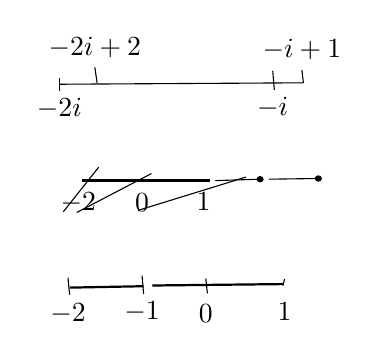
\begin{tikzpicture}[x=1cm,y=.9cm]
\draw (0,0)--(3.1,.02);
\draw (0,-.09)--(0,.09) node[below=4pt] {$-2i$};
\draw (.48,.02)--(.45,.24) node[above] {$-2i+2$};
\draw (2.73,-.08)--(2.71,.19) node[below=6pt] {$-i$};
\draw (3.1,.02)--(3.08,.2) node[above] {$-i+1$};
\draw[very thick] (.29,-1.36)--(1.91,-1.36);
\draw (1.98,-1.36)--(2.55,-1.34) (2.66,-1.34)--(3.29,-1.33);
\fill (2.55,-1.34) circle (.045) (3.29,-1.33) circle (.045);
\node at (.24,-1.67) {$\deleted{\unsure{-2}}$};
\node at (1.05,-1.67) {$\deleted{\unsure{0}}$};
\node at (1.83,-1.66) {$\deleted{\unsure{1}}$};
\draw (.05,-1.8)--(.5,-1.17) (.22,-1.81)--(1.17,-1.26)
 (1.00,-1.78)--(2.37,-1.31);
\draw[thick] (.13,-2.87)--(1.07,-2.85) (1.18,-2.84)--(2.85,-2.82);
\draw (.13,-2.97)--(.11,-2.73) node[below=6pt] {$-2$};
\draw (1.07,-2.96)--(1.05,-2.70) node[below=6pt] {$-1$};
\draw (1.88,-2.95)--(1.86,-2.74) node[below=6pt] {$0$};
\draw (2.84,-2.84)--(2.86,-2.75) node[below=5pt] {$1$};
\end{tikzpicture}} % 15–17
% archive sheet number: 72
\scanpage{74}
\mspage{\uline{16}}
Relations avec les pts \deleted{\unsure{d'ordre|d'}} rationnels \inserted{et la cohomologie} des % 1
Variétés abéliennes sur un \deleted{corps de fonctions} \inserted{schéma de type fini} \ldots % 2

Soit $A_K$ \unsure{VA|NA} sur corps $K$ de \uline{type fini} % 3
pour commencer. Alors $K$ est le corps des % 4
fonctions d'un schéma $\deleted{\unsure{X}}S$ irréductible et % 5
régulier, de type fini sur $\mathbb{Z}$, et \inserted{tel que} $A_K$ % 6
provient d'un schéma abélien sur $\deleted{\unsure{X}}S$. % 7

De plus, on a % 8
\[
 A_K(K)=A(\deleted{\unsure{X}}S) % 9
\]
et on sait que c'est un \uline{groupe de type % 10
fini} par Mordell-Weil-Néron-Lang. % 11

Soit $f:A\longrightarrow S$ la projection, et % 12
considérant le motif $\mathbb{R}^1 f^{*}_*(\mathbb{Q}_{A^*}(\deleted{\unsure{0}}1))\simeq
\deleted{\unsure{H_1(A)_{\mathbb{Q}}}} \inserted{T_{\text{\unsure{motif|mot}}}(A)}$ % 13
\inserted{[où $A^*$ est le dual de $A$]} % 14
qui est un motif ct tordu sur $S$ \deleted{de} % 15
pur de poids $1$, qui redonne $A_K$ % 16
\deleted{\unsure{à}} isogénie près \deleted{\unsure{sur $K$}} \deleted{\unsure{sur}} (sur $K$ ?) comme % 17
conséquence des conjectures de Tate. % 18
% archive sheet number: 73
\scanpage{75}
On s'attend donc à pouvoir écrire % 1
$A(S)\otimes_{\mathbb{Z}}\mathbb{Q}$ en termes de ce motif $M$. % 2
Or en effet, des \unsure{considérations|considér.|raisons} heuristiques convaincantes % 3
\deleted{pour} nous suggèrent % 4
\[
 A(S)\otimes_{\mathbb{Z}}\mathbb{Q}\simeq H^1(S,T_{\mathrm{mot}}(A)) % 5
\]
[NB. On doit avoir $H^0(S,T_{\mathrm{mot}}(A))=0$, % 6
à cause de \deleted{Mordell-Weil} considérations de % 7
poids ---- ]. \deleted{Une autre façon de} \inserted{Considérons} (pour $\ell$ premier % 8
aux car. résiduelles \unsure{de|à} $X$) % 9
\[
 \unsure{\varnothing|0}\longrightarrow{}_{\ell^\nu}A\longrightarrow A\longrightarrow A\;-\;0 % 10
\]
d'où % 11
\[
 0\longrightarrow H^0(S,A)_{\ell^\nu}\longrightarrow H^1(S,{}_{\ell^\nu}A)
 \longrightarrow{}_{\ell^\nu}H^1(S,A)\;\unsure{-|\to}\;0 % 12
\]
et par passage à la limite et $\otimes_{\mathbb{Z}_\ell}\mathbb{Q}_\ell$ % 13
\[
\begin{aligned}
0\longrightarrow {}&
\underbrace{H^0(S,A)}_{\substack{\text{de type fini}\\\text{sur }\mathbb{Z}}}
\otimes_{\mathbb{Z}}\deleted{\unsure{\mathbb{Z}|\mathbb{Q}}}\mathbb{Q}_\ell
 \longrightarrow H^1(S,T_{\ell}^{\deleted{\unsure{\mathbb{Q}}}}(A))_{\mathbb{Q}_\ell}
 \longrightarrow T_{\unsure{\bullet|\ell}}^{\deleted{\unsure{\mathbb{Q}}}}(H^1(S,A))_{\mathbb{Q}_\ell}\to0\\ % 14
&\hspace{36mm}\rotatebox{90}{$\simeq$}\\ % 15
&\hspace{32mm}H^1(S,T_{\mathrm{mot}}(A))\otimes_{\mathbb{Q}}\mathbb{Q}_{\ell}
\end{aligned} % 16
\]
et le résultat escompté ici équivaut % 17
moralement à celui-ci : % 18
\[
\boxed{\begin{aligned}
H^1(S,A)(\ell)\quad\text{\uuline{fini}}\qquad&\text{si }\ell\ \text{\textquotedblleft premier à } \deleted{\unsure{X}}S\text{\textquotedblright}\\ % 19
&\text{(}S\text{ de type fini sur }\operatorname{Spec}\mathbb{Z}\text{)}
\end{aligned}} % 20
\]
p.ex. si $S=\operatorname{Spec}\mathbb{F}_q$, alors c'est vrai par Lang ! % 21
% archive sheet number: 74
\scanpage{76}
Si $S$ est de type fini sur $\mathbb{F}_p$, on % 1
aura (travaillant avec des \uline{faisceaux % 2
étales}) si $f:S\longrightarrow\operatorname{Spec}\mathbb{F}_p$ % 3
\[
\begin{aligned}
0\to H^1(\mathbb{F}_p,R^0f_*A)\to H^1(S,A)\longrightarrow {}&
 H^0(\mathbb{F}_p,\mathbb{R}^1f_*(A))\longrightarrow0
 \deleted{\unsure{H^2(\mathbb{F}_p,R}}\\ % 4
&\rotatebox{90}{$=$}\\
&H^1(\bar S,\bar A)^\pi % 5
\end{aligned}
\]
Or on a, \unsure{tjrs|tjous|toujours} par \textquotedblleft Kummer\textquotedblright % 6
\[
\begin{aligned}
&\quad\inserted{M\otimes\mathbb{Q}_\ell/\mathbb{Z}_\ell}\\ % 7
0\to{}&H^0(\bar S,\bar A)\unsure{\otimes}\mathbb{Q}_\ell/\mathbb{Z}_\ell
 \;\unsure{-|\to}\; H^1(\bar S,{}_{\ell^\infty}\bar A)
 \to H^1(\bar S,\bar A)(\ell)\to0 % 8
\end{aligned}
\]
d'où le fait que $H^1(\bar S,\bar A)(\ell)$ est de % 9
poids $1-1=0$ \inserted{si p.ex. $S$ est projectif lisse sur $\mathbb{F}_p$} -- à priori rien ne s'oppose % 10
à ce qu'il y ait un gros module % 11
d'invariants. D'autre part, on a % 12
\[
\begin{aligned}
0\to &A^{\text{\unsure{fixe|fix}}}\longrightarrow R^0f_*(A)\longrightarrow M\longrightarrow 0\\ % 13
&\text{partie fixe}\hspace{29mm}\pi\text{-module,}\\ % 14
&\text{de la V.A. }A\text{ sur }S\hspace{12mm}\text{de type fini sur }\mathbb{Z}
\end{aligned} % 15
\]
d'où % 16
\[
\begin{aligned}
H^1(\mathbb{F}_p,A^{\text{fixe}})&\longrightarrow H^1(\mathbb{F}_p,\mathbb{R}^0f_*\unsure{M|A})
 \longrightarrow H^1(\mathbb{F}_p,M)\to0\\ % 17
\rotatebox{90}{$=$}\qquad&\hspace{46mm}\rotatebox{90}{$=$}\\
0\qquad&\hspace{35mm}(\unsure{\underline M|M}\otimes\mathbb{Q}/\mathbb{Z})^\pi\\ % 18
\text{par Lang}\qquad&
\end{aligned} % 19
\]
% archive sheet number: 75
\scanpage{77}
si $S$ de type fini sur $\mathbb{F}_p$, on obtient % 1
le diagramme suivant % 2
\diagram{\begin{tikzcd}[ampersand replacement=\&,column sep=small,row sep=small,font=\scriptsize]
\& \& M^\pi\otimes\mathbb{Q}_\ell/\mathbb{Z}_\ell \arrow[d,"{\rotatebox{90}{$\simeq$}}"{description},draw=none] \& \& \& \\ % 3
\& 0\arrow[r] \& H^0(S,A)\otimes\mathbb{Q}_\ell/\mathbb{Z}_\ell\arrow[r]\arrow[d]
\& H^1(S,{}_{\ell^\infty}A)\arrow[r]\arrow[d,two heads]
\& H^1(S,A)(\ell)\arrow[r]\arrow[d] \& 0\\ % 4
(1) \& 0\arrow[r] \& (H^0(\bar S,\bar A)\otimes\mathbb{Q}_\ell/\mathbb{Z}_\ell)^\pi\arrow[r]\arrow[d,"{\rotatebox{90}{$\simeq$}}"{description},draw=none]
\& H^1(\bar S,{}_{\ell^\infty}\bar A)^\pi\arrow[r]
\& H^1(\bar S,\bar A)(\ell)^\pi\arrow[r] \& 0\\ % 5
\& \& (M\otimes\mathbb{Q}_\ell/\mathbb{Z}_\ell)^\pi \& \& \&
\end{tikzcd}} % 6

[où $M=H^0(\bar S,\bar A)/H^0(\overline{\mathbb{F}}_p,\bar A^{\text{fixe}})$, % 7
$\pi$ est le gpe de Galois de $\overline{\mathbb{F}}_p$ sur $\mathbb{F}_p$] % 8

Les déterminations $H^0(S,A)\simeq M^\pi$ et $H^0(\bar S,\bar A)\otimes\mathbb{Q}_\ell/\mathbb{Z}_\ell$ % 9
$\simeq M\otimes\mathbb{Q}_\ell/\mathbb{Z}_\ell$ sont standart ; on voit que % 10
la première flèche verticale est un % 11
isomorphisme mod groupes finis. D'autre part, % 12
on trouve (suite spectrale de Leray de % 13
$f:S\to\operatorname{Spec}\mathbb{F}_p$ pour la \uline{top. étale}) % 14
\[
\begin{aligned}
0\to H^1(\mathbb{F}_p,R^0 f_*(A))&\to H^1(S,A)\to H^0(\mathbb{F}_p,R^1f_*(A))\to0\\ % 15
\rotatebox{90}{$\simeq$}\qquad&\hspace{28mm}\rotatebox{90}{$=$}\\
\text{groupe fini}\qquad&\hspace{24mm}H^1(\bar S,\bar A)_{\deleted{\unsure{\pi}}}^{\pi}
\end{aligned} % 16
\]
$\lhook\joinrel\longrightarrow$ comme on voit utilisant % 17
\[
0\to\bar A^{\text{fixe}}\to R^0f_*(A)\to M\to0\,,\qquad\text{et les} % 18
\]
% archive sheet number: 76
\scanpage{78}
\margin{\tikz[baseline=-.3ex]{\draw (0,0) circle (.035) (0,.03)--(.30,.52);}} % slanted
$H^2(S,A)$ \deleted{\unsure{de} $H^2$} (dont le $T_\ell$ est $H^2(S,T_\ell(A))$) % 1
n'est pas néc nul, \deleted{\unsure{si}} \inserted{comme on voit} si $S$ est % 2
une courbe lisse projective géom connexe sur $\mathbb{F}_p$, % 3
et $A=J\times S$, où $J$ est la jacobienne de $S$. % 4
On a en tous cas % 5
\[
\begin{aligned}
 H^2(S,T_\ell(A)) &\simeq \unsure{\mathbb{H}|H}^{1}(\bar S,T_\ell(\bar A))_{\pi}
 =\deleted{T_\ell J(\overline{\mathbb{F}}_p)\otimes}
 \inserted{\bigl[T_\ell(\bar J)\otimes T_\ell(\bar J)\bigr]_{\pi}}\\ % 6
 &\simeq\operatorname{End}(J)\otimes_{\deleted{\unsure{\mathbb{Q}}}\mathbb{Z}}\mathbb{Q}_{\ell}
 \quad\deleted{\text{\unsure{qui}}}\bigl(\simeq
 \bigl(\text{\unsure{Algèbre|classes} de corr. }\inserted{\text{\unsure{divisorielles}}}\text{ sur la }C\bigr)
 \otimes_{\mathbb{Z}}\mathbb{Q}_{\ell} % 7
\end{aligned}
\]
qui est non nul ----. % 8
% archive sheet number: 77
\scanpage{79}
que $H^1(\mathbb{F}_p,A^{\text{fixe}})=0$ (Lang) et % 1
$H^1(\mathbb{F}_p,M)=\text{fini}$ [trivial ; Attention qu'il s'agit % 2
de la coh. \uline{étale}, i.e la coh. \uline{galoisienne} de % 3
$\widehat{\mathbb{Z}}$ !], donc la dernière flèche verticale % 4
du diagramme $(1)$, est aussi bijective : % 5
\[
H^1(S,A)(\deleted{\unsure{p}}\ell)\xrightarrow{\sim}H^1(\bar S,\bar A)^\pi(\ell)
 \qquad\text{\uline{surj à noyau fini} ---} % 6
\]
Donc la \uline{conjecture} précédente signifie aussi % 7
\[
\boxed{H^1(\bar S,\bar A)(\ell)^\pi=\text{groupe fini}} % 8
\]

\deleted{Il y a une façon de \unsure{le|la} prouver,} % 9

C'est \inserted{aussi} $\pm$ équiv. (via des jacobiennes) à % 10
ceci : $X\longrightarrow S$ morphisme propre [lisse % 11
de dim relative $1$], $S$ régulier de % 12
type fini sur $\mathbb{Z}$. Prouver que % 13
$H^2(S,G_m)\longrightarrow H^{\unsure{2|1}}(X,G_m)$ est surjectif mod % 14
groupes finis ?? % 15
\margin{$\nwarrow$ \tikz[baseline=-.3ex]{\draw (0,0) circle (.035) (0,.03)--(.30,.52);}} % slanted

\margin{donc les seuls \unsure{inv.|invar.} qui restent sont $H^0$ et $H^2$ pour $A$, et \deleted{$\unsure{H^0}$}, $H^1$, $H^2$ pour $T_\ell(A)$} % slanted
\uline{NB} On devrait avoir $H^{\deleted{\unsure{2}}i}(S,A)(\ell)$ fini aussi % 16
pour \uuline{$i\ge3$}, $S$ de type fini sur $\mathbb{Z}$, $\ell$ premier aux % 17
car. résiduelles \unsure{de $S$|à ----|-----} (\inserted{NB} si $i\ge2$, $T_\ell(H^i(S,A)(\ell))\simeq H^i(S,T_\ell(A))$) % 18
% archive sheet number: 78
\scanpage{80}
Noter que % 1
\[
H^1(S,\deleted{\unsure{A|T}}T_\ell(A))\simeq H^1(\bar S,\unsure{T_\ell\bar A)|T_\ell(\bar A)})^\pi % 2
\]
Donc notre conjecture signifie \unsure{essentiellem\textsuperscript{t}|essentiellement} % 3
\[
\operatorname{rang}_{\mathbb{Q}_\ell}\bigl(H^1(\bar S,T_\ell(\bar A)\bigr)^\pi
 \simeq \operatorname{rang}_{\mathbb{Z}} A(K) % 4
\]
et sous cette forme est \unsure{essentiellem\textsuperscript{t}|essentiellement} % 5
équivalente à la \uline{conjecture de} % 6
\deleted{\unsure{Swinn|Serre}} \uline{Birch - \unsure{Swinnerton|Swinnertun}-Dyer.} % 7
% archive sheet number: 79
